\documentclass[tikz, border=1mm]{standalone}
\usetikzlibrary{arrows, shapes.gates.logic.US, calc}
\begin{document}
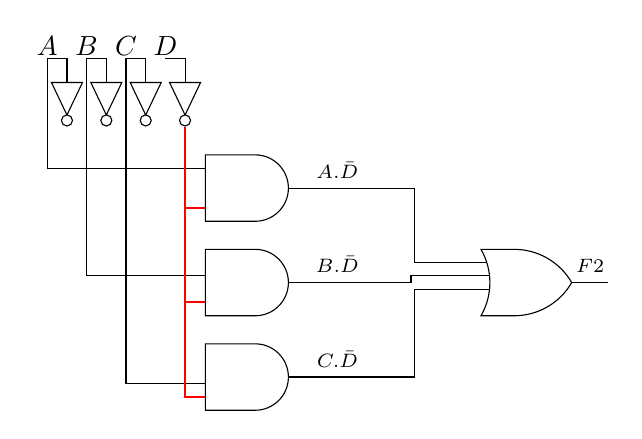
\begin{tikzpicture}

 %%Paramaters
%% var position, can be modified
\def\varPos{19.80}
\def\FunctionPos{6}
\node (x) at (0, \varPos) {$A$};
\node (y) at (0.5, \varPos) {$B$};
\node (z) at (1, \varPos) {$C$};
\node (w) at (1.5, \varPos) {$D$};

                \node[not gate US, draw, rotate=270] at ($(x) + (0.25, -0.6)$) (notx) {};
                \draw ($(x)+(0,-1ex)$) -| (notx.input); 
                \node[not gate US, draw, rotate=270] at ($(y) + (0.25, -0.6)$) (noty) {};
                \draw ($(y)+(0,-1ex)$) -| (noty.input); 
                \node[not gate US, draw, rotate=270] at ($(z) + (0.25, -0.6)$) (notz) {};
                \draw ($(z)+(0,-1ex)$) -| (notz.input);
                \node[not gate US, draw, rotate=270] at ($(w) + (0.25, -0.6)$) (notw) {};
                \draw ($(w)+(0,-1ex)$) -| (notw.input);



 %% ***Function F2 : Gate for term n° 1 [ C.D' ]***
  
                \node[and gate US, draw, rotate=0, logic gate inputs=nnnn] at (2.5, 15.60) (xandy13) {};\draw (xandy13.output) -- node[above]{\scriptsize $ C.\bar D $} ($(xandy13) + (1.8, 0)$);
                % Z
\draw ($(z) + (0, -1ex)$)|- (xandy13.input 3);
% W
\draw [line width=0.25mm,   red] (notw.output)
            -- ([xshift=0cm]notw.output) |- (xandy13.input 4);
 

 %% ***Function F2 : Gate for term n° 2 [ B.D' ]***
  
                \node[and gate US, draw, rotate=0, logic gate inputs=nnnn] at (2.5, 16.80) (xandy14) {};\draw (xandy14.output) -- node[above]{\scriptsize $ B.\bar D $} ($(xandy14) + (1.8, 0)$);
                % Y
\draw ($(y) + (0, -1ex)$)|- (xandy14.input 2);
% W
\draw [line width=0.25mm,   red] (notw.output)
            -- ([xshift=0cm]notw.output) |- (xandy14.input 4);
 

 %% ***Function F2 : Gate for term n° 3 [ A.D' ]***
  
                \node[and gate US, draw, rotate=0, logic gate inputs=nnnn] at (2.5, 18.00) (xandy15) {};\draw (xandy15.output) -- node[above]{\scriptsize $ A.\bar D $} ($(xandy15) + (1.8, 0)$);
                % X
\draw ($(x) + (0, -1ex)$)|- (xandy15.input 1);
% W
\draw [line width=0.25mm,   red] (notw.output)
            -- ([xshift=0cm]notw.output) |- (xandy15.input 4);


%% Function F2 Large OR Gate

\node[or gate US, draw, rotate=0, logic gate inputs=nnnn] at (\FunctionPos, 16.80) (xory13) {};


            \draw (xory13.output) -- node[above]{\scriptsize $F2$} ($(xory13.east) + (+3ex, 0)$);


            \draw (xandy13.output) -- ([xshift=1.60cm]xandy13.output) |- (xory13.input 3);

\draw (xandy14.output) -- ([xshift=1.55cm]xandy14.output) |- (xory13.input 2);

\draw (xandy15.output) -- ([xshift=1.60cm]xandy15.output) |- (xory13.input 1);
 \end{tikzpicture}
         \end{document}
